\documentclass{scrartcl}

\usepackage[utf8]{inputenc}
\usepackage[T1]{fontenc}
\usepackage{lmodern}

\usepackage[sc]{mathpazo} % or option osf
\usepackage{newpxmath}

%\usepackage[comma,authoryear]{natbib}
\bibliographystyle{plain}

\usepackage{adjustbox}
\usepackage[a4paper, margin=1mm, includefoot, footskip=15pt]{geometry}

\usepackage[pdftitle={Global country borders extracted from open street map}
, pdfauthor={Georg Kindermann}
, pdfsubject={county borders, administrative borders, global}
, pdfkeywords={borders, global, county, administrative, osm, open street map}
, pdflang={en-UK}
, hidelinks
, pdfpagemode=None]{hyperref}

\nonfrenchspacing
\sloppy

\title{Global country borders extracted from open street map}
\author{Georg Kindermann}

\begin{document}

\maketitle

The maps of open street map (OSM) contain country borders. The data
can be accesses at \cite{osmPlanet}. With \cite{andGem} boundary
polygons could be extracted. Those have been joined together with
\cite{GRASS_GIS_software} and ISO country codes form \cite{wikiIso}
have been added using \cite{sqlite2020hipp}. Splitting up to single
countries was done with \cite{QGIS_software} and format conversions
was done with \cite{gdal}.

\begin{figure}[htbp]
  \centering
  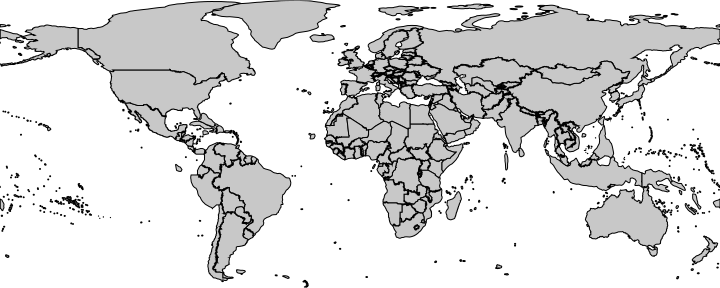
\includegraphics[width=.9\linewidth]{map.png}
  \caption{Country border of OSM in 2000--01--06}
  \label{fig:map}
\end{figure}

A file in GeoPackage format with global coverage and single files for
each county are provided.\\
Currently for 2000--01--06.\\
Each country polygon gives the information:

\begin{tabular}{lllll}
  name & iso2 & iso3 & isoNr & namee\\
  \hline
Andorra & AD  & AND  &    20 & Andorra\\
Angola  & AO  & AGO  &    24 & Angola\\
\end{tabular}

\begin{description}
\item[name] Country name as given in OSM
\item[iso2] Two--letter country codes (ISO 3166-1 alpha-2)
\item[iso3] Three--letter country codes (ISO 3166-1 alpha-3)
\item[isoNr] Three-digit country codes (ISO 3166-1 numeric)
\item[namee] English country name as given in \cite{wikiIso}
\end{description}

The data can be accessed at
\url{https://user.iiasa.ac.at/~kinder/gfd/countryBorders/} in the
\href{https://iiasa.ac.at/models-and-data/global-forest-database}{Global
  Forest Database}.

\bibliography{literature}

%Autor: Georg Kindermann

\end{document}
